\documentclass[a4paper,11pt]{article}
\usepackage{jheppub} % for details on the use of the package, please see the JINST-author-manual
% \usepackage{lineno}
% \linenumbers

\usepackage[symbol]{footmisc}
\usepackage{amssymb,tabularx,amsmath}
\usepackage{tikz}
\usetikzlibrary{arrows.meta, positioning}

%  \usepackage{mathtools}
% \DeclarePairedDelimiter\bra{\langle}{\rvert}
% \DeclarePairedDelimiter\ket{\lvert}{\rangle}
% \DeclarePairedDelimiterX\braket[2]{\langle}{\rangle}{#1\,\delimsize\vert\,\mathopen{}#2}
\makeatletter
\usepackage{braket}
\renewcommand{\thefootnote}{{\@arabic\c@footnote}}
\newcommand{\omegap}{\omega'}
\newcommand{\betaok}{\beta_{\omega k}}
\newcommand{\alphaok}{\alpha_{\omega k}}
\newcommand{\betaopk}{\beta_{\omega' k}}
\newcommand{\alphaopk}{\alpha_{\omega' k}}
\newcommand{\vv}{\mathbb{V}}
\newcommand{\norm}[1]{\left\lVert#1\right\rVert}
\newcommand{\iminus}{$i^-$}
\newcommand{\iplus}{$i^+$}
\newcommand{\coordt}{$t$}
\newcommand{\coordz}{$z$}
\newcommand{\scrim}{$\mathcal{I}^-$}
\newcommand{\scrip}{$\mathcal{I}^+$}
\newcommand{\dl}{\partial}
\newcommand{\inz}{\mathcal{Z}}

\arxivnumber{1234.12345} % if you have one

\title{\boldmath Particle spectrum in Moving Mirror Problem using Deep learning techniques}

% Collaborations

%% [A] If main author
%% \collaboration{\includegraphics[height=17mm]{collabroation-logo}\\[6pt]
%%  XXX collaboration}

%% or
%% [B] If "on behalf of"
%% \collaboration[c]{on behalf of XXX collaboration}


% Authors
% The "\note" macro will give a warning: "Ignoring empty anchor...", you can safely ignore it.

%% [A] simple case: 2 authors, same institution
%% \author[1]{A. Uthor\note{Corresponding author.}}
%% \author{and A. Nother Author}
%% \affiliation{Institution,\\Address, Country}

%% or, e.g.
%% [B] more complex case: 4 authors, 3 institutions, 2 footnotes
%% \author[a,b]{F. Irst,\note{Now at another university}}
%% \author[c]{S. Econd,}
%% \author[a,2]{T. Hird\note{Also at Some University.}}
%% \author[c,2]{and Fourth}
%% \affiliation[a]{Institution_1,\\Address, Country}
%% \affiliation[b]{Institution_2,\\Address, Country}
%% \affiliation[c]{Institution_3,\\Address, Country}

\author{A. Uthor}
\affiliation{One University,\\
some-street, Country}
\affiliation{Another University,\\
different-address, Country}

% E-mail addresses: only for the corresponding author
\emailAdd{first@one.univ}

\abstract{Abstract...}



\begin{document}
\maketitle
\flushbottom
% 
\section{Introduction}
\label{sec:intro}

For internal references use label-refs: see section~\ref{sec:intro}.
Bibliographic citations can be done with "cite": refs.~\cite{a,b,c}.
When possible, align equations on the equal sign. The package
\texttt{amsmath} is already loaded. See \eqref{eq:x}.
\begin{equation}
\label{eq:x}
\begin{aligned}
x &= 1 \,,
\qquad
y = 2 \,,
\\
z &= 3 \,.
\end{aligned}
\end{equation}
Also, watch out for the punctuation at the end of the equations.


If you want some equations without the tag (number), please use the available
starred-environments. For example:
\begin{equation*}
x = 1
\end{equation*}

\section{Figures and tables}

All figures and tables should be referenced in the text and should be
placed on the page where they are first cited or in
subsequent pages. Positioning them in the source file
after the paragraph where you first reference them usually yield good
results. See figure~\ref{fig:i} and table~\ref{tab:i} for layout examples. 
Please note that a caption is mandatory  and it must be placed at the bottom of both figures and tables.

\begin{figure}[htbp]
\centering
\includegraphics[width=.4\textwidth]{example-image-a}
\qquad
\includegraphics[width=.4\textwidth]{example-image-b}
\caption{Always give a caption.\label{fig:i}}
\end{figure}

\begin{table}[htbp]
\centering
\begin{tabular}{lr|c}
\hline
x&y&x and y\\
\hline
a & b & a and b\\
1 & 2 & 1 and 2\\
$\alpha$ & $\beta$ & $\alpha$ and $\beta$\\
\hline
\end{tabular}
\caption{We prefer to have top and bottom borders around the tables.\label{tab:i}}
\end{table}

We discourage the use of inline figures (e.g. \texttt{wrapfigure}), as they may be
difficult to position if the page layout changes.

We suggest not to abbreviate: ``section'', ``appendix'', ``figure''
and ``table'', but ``eq.'' and ``ref.'' are welcome. Also, please do
not use \texttt{\textbackslash emph} or \texttt{\textbackslash it} for
latin abbreviaitons: i.e., et al., e.g., vs., etc.


\paragraph{Up to paragraphs.} We find that having more levels usually
reduces the clarity of the article. Also, we strongly discourage the
use of non-numbered sections (e.g.~\texttt{\textbackslash
  subsubsection*}).  Please also consider the use of
``\texttt{\textbackslash texorpdfstring\{\}\{\}}'' to avoid warnings
from the \texttt{hyperref} package when you have math in the section titles.



\section{Introduction}
The setup of the system and the calculations it follows are heavily borrowed from \cite{Obadia_2001}. Our focus lies completely in the section (2.1), and we do not bother ourselves with the partially reflecting mirror case.
%%%%%%%%%%%%%%%%%%%%%%%%%%%%%%%%%%%%%%%%%%%%%%%%%%%%%%%%%%%%%%%%%%%%%%%%%%%%%%%%%%%%%%%%%%%%%%%%%%%%

\section{Penrose diagram for 1+1 dimension}

To formulate the Penrose diagram, we consider various limits of the coordinates to reach different asymptotic regions of the spacetimes. We begin with the coordinates (\coordt,\coordz) but since the focus lies on massless scalar field in 2 dimension, we formulate our problem in the light cone coordinate which are given as $U, V~=~ t\mp z$.
 

The Penrose diagrams for the following can be seen as 
\begin{figure}
    \centering
    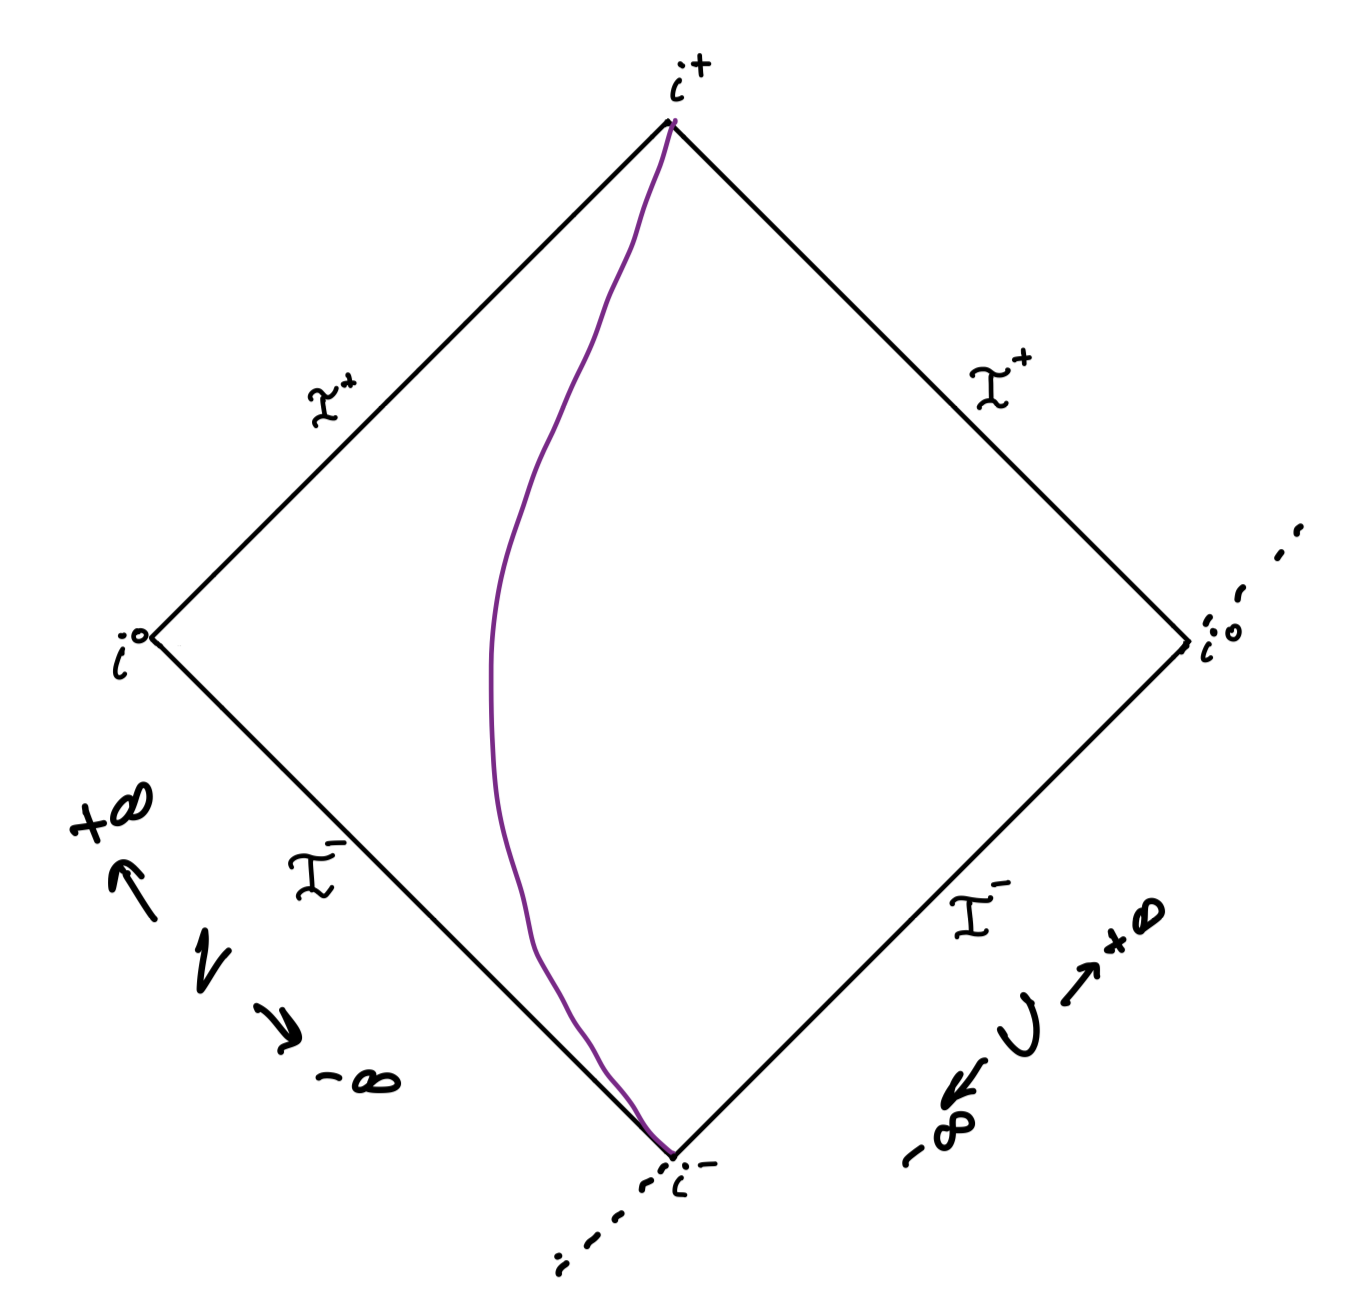
\includegraphics[width=0.5\linewidth]{Penrose diagram.png}
    \caption{Penrose Diagram 1+1}
    \label{fig:penrose_diagram}
\end{figure}
The construction of the above diagram can be seen in the appendix \ref{app:PenDiag}
%----------------------------------------------------------------------------------------------------------------------------------------

\section{Real Scalar field}

The setup of the problem is as follows: There is a point mirror whose trajectory starts from \iminus and ends at \iplus. A scalar that satisfies the massless Klein-Gordon equation
\begin{equation}\label{eq:waveequationtr}
    (\frac{\partial^2}{\partial t^2}-\frac{\partial^2}{\partial z^2})\Phi(t,z)~=~0
\end{equation}

or

\begin{equation*}\label{eq:waveequationUV}
    \frac{\partial^2}{\partial U\partial V}\Phi(U,V)~=~0
\end{equation*}
 is emitted from the past null infinity and after getting scattered off the mirror reaches future null infinity. Since, we are not considering the back reaction of scattering in this problem, the motion of mirror can be specified freely. Also, since the mirror is a massive object, the trajectory of the mirror starts from \iminus and ends at \iplus. Let the trajectory of the mirror is given by $z_{cl}(t)$.
 
 
 Because the mirror is perfectly reflecting we impose the boundary condition
 \begin{equation}\label{eq:bc}
    \Phi(t,z_{cl}(t))~=~0    
 \end{equation}

 Also, the left modes completely decouple from the right modes as can be seen from the general solution of the wave equation. We here focus on the field which live on the left hand side of the mirror(\ref{fig:penrose_diagram})\. The solution to equation (\ref{eq:waveequationUV}) on the surface V = -$\infty$ is 
 \begin{equation}\label{eq:modeU}
    \varphi_k(U)~=~\frac{e^{-i k U}}{\sqrt{4\pi|k|}}.
 \end{equation}

 Above modes form a complete and orthonormal basis of the equation (\ref{eq:waveequationUV}). They are orthogonal in the sense of the norm determined by the Klein-Gordon scalar product, which reads, when evaluated on \scrim :
 \begin{equation}\label{eq:KG_inner_product}
    \braket{\varphi_k|\varphi_{k'}}~=~\int^{+\infty}_{-\infty}dU i(\varphi^*_k\dl_U\varphi_{k'}-\varphi_{k'}\dl_U\varphi^*_k)
 \end{equation}
Let us check the above expression for two modes given in \ref{eq:modeU}.
\begin{equation}\label{eq:orthorr}
\begin{aligned}
     \braket{\varphi_k|\varphi_{k'}}~&=~\int^{+\infty}_{-\infty}dU i(\varphi^*_k\dl_U\varphi_{k'}-\varphi_{k'}\dl_U\varphi^*_k)\\
    &=~\int^{+\infty}_{-\infty}dU i\left(\frac{e^{i k U}}{\sqrt{4\pi|k|}}\dl_U(~\frac{e^{-i k' U}}{\sqrt{4\pi|k'|}})-~\frac{e^{-i k' U}}{\sqrt{4\pi|k'|}}\dl_U(~\frac{e^{i k U}}{\sqrt{4\pi|k|}})\right)\\
    &=~\int^{+\infty}_{-\infty}dU i\left(\frac{e^{i k U}}{\sqrt{4\pi|k|}}(-ik')~\frac{e^{-i k' U}}{\sqrt{4\pi|k'|}}-~\frac{e^{-i k' U}}{\sqrt{4\pi|k'|}}(ik)~\frac{e^{i k U}}{\sqrt{4\pi|k|}}\right)\\
    &=~\int^{+\infty}_{-\infty}dU\frac{e^{iU(k-k')}}{\sqrt{4\pi|k|}\sqrt{4\pi|k'|}}(k'+k)\\
    &=~\frac{(k'+k)}{\sqrt{4\pi|k|}\sqrt{4\pi|k'|}}\int^{+\infty}_{-\infty}dU e^{iU(k-k')}\\
    &=~\frac{(k'+k)}{4\pi\sqrt{|k||k'|}}2\pi\delta(k-k')\\
    &=~\frac{2k}{2\sqrt{|k||k'|}}\delta(k-k')\\
    &=~\emph{sgn(k)}\delta(k-k')
\end{aligned}
\end{equation}
The other related quantities are as follows,
\begin{enumerate}
    \item $<\varphi^*_k|\varphi^*_{k'}>~=~\emph{sgn(k)}\delta(k-k')$,
    \item $<\varphi^*_k|\varphi_{k'}>~=~-~\emph{sgn(k)}\delta(k+k')$.
\end{enumerate}
The calculation of the above can be found in the Appendix \ref{app:IPmode}

The value of the scalar field, as given by the solution, on the mirror is 
 \begin{equation*}
     \varphi_k^{scat}(V)~=~\frac{e^{-i k U_{cl}(V)}}{\sqrt{4\pi|k|}}
 \end{equation*}.
 Let's look at the quantity $U_{cl}$ quickly. In order to obtain it, we look at the coordinate transformation, $U, V~=~t\mp z$. For $V_{cl}=t~-~z_{cl}(t)$, we assume that in principle, one can always invert this relation (at least numerically) in the form, $t~=~f(V_{cl})$. Then we substitute this equation in the $U$ relation, $U_{cl}(V)~=~f(V)+z_{cl}(f(V))$.

 
 Finally, the in-mode $\varphi_k^{in}(U,V)$ is given by 
 \begin{equation*}
     \varphi_k^{in}(U,V) = \frac{e^{-i k U}}{\sqrt{4\pi|k|}}-\frac{e^{-i k U_{cl}(V)}}{\sqrt{4\pi|k|}}
 \end{equation*}
Above given in-mode is the solution of our system \ref{eq:waveequationtr}, which follows the boundary condition \ref{eq:bc}
 To analyse the frequency content of its scattered part, it should be Fourier decomposed on the final Cauchy surface $U~=~+\infty$. In total analogy with what we have on \scrim, on \scrip we have 
 \begin{equation*}
     \varphi_\omega(V)~=~\frac{e^{-i \omega V}}{\sqrt{4\pi|\omega|}}.
 \end{equation*}

 The scattered mode can be decomposed as 
 \begin{equation*}
     \varphi_k^{scat} = \int_0^\infty d\omega(\alpha^*_{\omega k}\varphi_\omega-\beta^*_{\omega k}\varphi_\omega^*),
 \end{equation*}
where the coefficients $\alpha_{\omega k}~,~\beta_{\omega k}$ are known as \emph{Bogoliubov coefficients}. They can be determined by the Klein-Gordon inner product by (\ref{eq: KG_inner_product}) as  
\begin{enumerate}
    \item $\alphaok^*~=~<\varphi_{\omega}|\varphi^{scat}_k>$
    \item $\betaok^*=<\varphi^*_{\omega}|\varphi^{scat}_k>$
\end{enumerate}
The explicit expression for the $\betaok$ can be computed as,
\begin{eqnarray}\label{eq:beta}
\begin{aligned}
    \betaok &=~ <\varphi_{\omega}|\varphi^{*scat}_k> \\
    &=\int_{-\infty}^{+\infty} dV i\left(\frac{e^{-i \omega V}}{\sqrt{4\pi|\omega|}}\dl_V(\frac{e^{i k U_{cl}(V)}}{\sqrt{4\pi|k|}})-\frac{e^{i k U_{cl}(V)}}{\sqrt{4\pi|k|}}\dl_V(\frac{e^{-i \omega V}}{\sqrt{4\pi|\omega|}})\right)\\
    % &=-\int_{-\infty}^{+\infty} dV i\left(\frac{e^{-i \omega V}}{\sqrt{4\pi|\omega|}}\dl_V(\frac{e^{-i k U_{cl}(V)}}{\sqrt{4\pi|k|}})-\frac{e^{-i k U_{cl}(V)}}{\sqrt{4\pi|k|}}\dl_V(\frac{e^{-i \omega V}}{\sqrt{4\pi|\omega|}})\right)\\
    &=\int_{-\infty}^{+\infty} dV i\left(\frac{e^{-i \omega V}}{\sqrt{4\pi|\omega|}}(ik\dl_VU_{cl}(V))(\frac{e^{i k U_{cl}(V)}}{\sqrt{4\pi|k|}})-\frac{e^{i k U_{cl}(V)}}{\sqrt{4\pi|k|}}(-i\omega)(\frac{e^{-i \omega V}}{\sqrt{4\pi|\omega|}})\right)\\
    &=\int_{-\infty}^{+\infty} dV \frac{e^{i(U_{cl}(V)k-V\omega)}}{\sqrt{4\pi|\omega|}\sqrt{4\pi |k|}}(-k\dl_V U_{cl}(V)-\omega)\\
    \end{aligned}
\end{eqnarray}

% A similar calculation for $\alphaok$ can be found in Appendix \ref{app:b_coeff}. In order to get the expression for $\alpha_{\omega k}$, let's look at the following quantity,

% \begin{eqnarray*}
%      &=~<\varphi_{\omegap}|\varphi^{scat}_k>\\
%      &=~ <\varphi_{\omegap}|\int_0^\infty d\omega(\alpha^*_{\omega k}\varphi_\omega-\beta^*_{\omega k}\varphi_\omega^*)>\\
%     &=~\int_0^\infty d\omega<\varphi_{\omegap}|(\alpha^*_{\omega k}\varphi_\omega-\beta^*_{\omega k}\varphi_\omega^*)>\\
%     &=~\int_0^\infty d\omega(\alpha_{\omega k}^*<\varphi_{\omegap}|\varphi_\omega>-\beta^*_{\omega k}<\varphi_{\omegap}|\varphi_\omega^*>)\\
%     &=~\int_0^\infty d\omega(\alpha_{\omega k}^*\emph{sgn}(\omega)\delta(\omega-\omegap)+\beta^*_{\omega k}\emph{sgn}(\omega)\delta(\omega+\omegap))\\
%     &=~\alpha^*_{\omegap k}
% \end{eqnarray*}

From the commutation relation of the two different modes, we can deduce the following relations
\begin{equation}\label{eq:constraints}
    \begin{aligned}
        \int_0^{\infty}dk (\alphaok^*\alpha_{\omega'k}-\betaok\beta_{\omega'k}^*)~&=~\delta(\omega'-\omega)\\
        \int_0^{\infty}d\omega (\alphaok\alpha_{\omega k'}^*-\betaok\beta_{\omega k'}^*)~&=~\delta(k'-k)\\
        \int_0^{\infty}dk (\alphaok\beta_{\omega k'}-\betaok\alpha_{\omega k'}^*)~&=~0\\
        \int_0^{\infty}d\omega (\alphaok\beta_{\omega' k}^*-\betaok^*\alpha_{\omega'k})~&=~0\\
    \end{aligned}
\end{equation}

As we will see, the above relation will vastly help us in generalising the output of the neural network away from the training data.

\color{red}
\subsection{Constraints}

Since, the neural operators approximates the function $\alphaok$, we need another neural network parallel to which also approximates $\betaok$. Since I now have them in the matrix form I can discretise the constraint equations to become matrix equations to be solved in a simple manner. Essentially the constraint equation is then
\begin{eqnarray*}
    \sum_{k=1}^{N}\frac{1}{N}(\alphaok^*\alphaopk-\betaok\betaopk^*)~=~\delta_{\omega,\omega'}
\end{eqnarray*}
In this simple way we can impose the constraints. Maybe the loss will look like
\begin{equation}
   \mathbb{C}_1=\norm{\sum_{k=1}^{N}\frac{1}{N}(\alphaok^*\alphaopk-\betaok\betaopk^*)~-~\delta_{\omega,\omega'} }
\end{equation}
The dirac delta which appears in the above equation is essentially a unit matrix if the discretisation of $\omega$ and $\omega'$ is same.

The function $\betaok$, is the focus of our work. One can see that the number operator calculated for the observer at \scrip, is given by

\begin{equation*}
    N_k=\int_{-\infty}^{+\infty}|\betaok|^2d\omega
\end{equation*}


% \section{Solving for $\betaok$}

% The function $\betaok$ is the key element while calculating the total energy of the field and the total number of particle, as experienced by one observer\cite{Good_2017,Good_2020}. We focus on engineering a neural network to approximate the function $\betaok$. Since the function $\betaok$ is parameterized by the two frequencies which are continuous, the only way to implement it on a computer is to discretise it. In doing so, $\betaok$ becomes a matrix of size $N\times N$. 

% The discretization of the frequency is to be done in a careful manner. Due to our restriction on the left moving modes only, the frequency spectrum in only limited to positive frequency. The domain of discretization and the number of  discretization points in the frequency domain do not affect the way we are trying to do the computations. To keep it simple, we will have uniform distribution and equal domain for both the frequencies. The abovementioned statement can be assumed to be true because the neural networks are found to interpolate well within the collocation domain. \textcolor{red}{Add few refernces on this.}

% \subsection{Neural Network Architecture}
 

%  As we have already convinced ourselves that the function $\betaok$ will be a matrix, the neural network is to be written in such a manner that the output should be a matrix. Such neural networks have been studied before \cite{gao2016matrixneuralnetworks}. 

% Consider an array that encodes the discretisation of the time domain,
% \begin{equation}
%     T~=~\left[t_1,t_2,...,t_N\right]^T.
% \end{equation}.

% Then, for a given trajectory of the mirror $z_{cl}(t)$, the trajectory is given by
% \begin{equation}
%     \inz~=~\left[z(t_1),z(t_2),...,z(t_N)\right]^T.
% \end{equation}
 
% In this way, $\inz$ becomes the input for our neural network. In section \ref{}, we will see how the training data is generated.

% A layer of the neural network is given as ,

% \begin{equation}
%     y^{(\mu+1)}_{ab} =     
%     \sigma(\sum_{c,d}W^{(\mu)}_{abcd}y^{(\mu)}_{cd}+b_{cd}^{(\mu)})
% \end{equation}
% , where $\sigma$ is an activation function which will be chosen to be \textcolor{red}{tanh(x)}. The index $\mu$ indicates the hidden layer. The rank of the weight matrix and basis is chosen in such a way that, even though the input layer is only a column vector the final output is a matrix.

% A few remarks are in order,
% \begin{enumerate}
%     \item In order to get $\betaok$ as output, we discretise the frequency domain, so that $\betaok$ become a matrix. The two frequencies will play the role of two indices of the matrix. The reason to do so is two fold. Firstly, when we obtain the two coefficients in matrix form then the implementation of the constraints simplifies to matrix multiplication.

%     In this way the first equation in \ref{eq:constraints} becomes 
%     \begin{equation*}
%          \sum_{k=1}^{N}\frac{1}{N}(\alphaok^*\alphaopk-\betaok\betaopk^*)~=~\delta_{\omega,\omega'}
%     \end{equation*}
%     or 
%     \begin{equation*}
%         \alpha^*\alpha^\intercal-\beta\beta^\dag =\mathbb{1}
%     \end{equation*}
%     \item The output of the model is supposed to be a complex matrix\cite{barrachina2023theoryimplementationcomplexvaluedneural,complex_IEEE,Dramsch_2021_complex}. There the theory of complex valued neural network has attracted attention recently because of a simple reason that almost every branch of engineering deals with complex numbers. Since the theory of holonomic functions is includes subtleties like branch cuts and poles, it is not straightforward to generalise a neural network to include complex numbers.  Inclusion of complex weights and biases in the model results in lots of choices that can be made for activation function. \\
%     Here, we will choose the simplest way to implement the above. The activation function acts independently on the real and imaginary part of the output of a neuron. The real and imaginary parts go through same initialisation scheme but again independently. This is the simplest way to deal with complex functions and not run into various subtelties.
    
% \end{enumerate}

% \section{Implementation}



% \subsection{Testing our neural network}
% We tested our modified architecture to fit the function $sin(x)$. First, we changed the layer structure to a $N \times N$ matrix, which leaves us with a $N \times N \times N \times N$ weight tensor $W$ and a $N \times N$ bias tensor $b$. The activation function used was $tanh(x)$ and the neurons, weights and biases can all take up complex values.

% For testing, we chose $N=4$ and the target function to be $Y = sin(AX+B)$, where X \& Y are the input and output matrices respectively and A \& B were chosen randomly.

% $$
%  A = \begin{pmatrix}
%   1.1998-0.1574j &  0.6373-0.5554j & -0.7039-1.0864j & 0.3819-1.3114j\\
%   0.0756-0.5395j & -0.0053-0.6152j & -0.8208-0.0869j & -1.9599+0.8681j \\
%   -0.4195-0.1863j & -0.2006+0.1367j & 0.1942+0.3467j & -1.0001+1.1453j\\
%   -0.3711-1.1124j & 0.1005+0.8200j & -0.4263-0.1863j &  1.6511+0.4498j\\
%  \end{pmatrix}
% $$
% $$
% B = \begin{pmatrix}
%     -0.6968-0.8846j & 0.7214-0.5691j & -0.9276-0.7205j &   0.1747+0.0385j\\
%     0.4997+1.1992j & 0.6392-1.1646j & 0.0002+0.1768j &        -0.3270+0.6001j\\
%     0.8354+0.7416j & 1.3680-0.0796j &  1.0705+0.2365j & 0.1610+0.2640j\\
%     1.1970+0.3054j & 1.4600+1.0038j & -0.4845+0.7547j &
%     0.1427-0.3385j\\
% \end{pmatrix}
% $$

% We then generated $100$ random $4\times 4$ matrices as training data for $X$ and calculated $Y = sin(AX+B)$. Our neural network had 2 layers, the optimizer chosen was "Adam" and Mean Squared Error (MSE) was chosen as the loss function. The neural network was trained on for 200 epochs and in the end, the training loss obtained was 69.4404.

% We then compared our neural network's prediction with the expected output for one randomly chosen $4 \times 4$ matrix and compared the results.

% $$Y_{pred} - Y_{actual} = \begin{pmatrix}
%     0.7403+1.3917j & -0.1595-0.0605j & 0.2038-0.26527j & 1.2080+0.0336j\\
%     5.1085+3.9645j & -0.8260+0.8135j &  0.6814-0.4258j &  2.9697+1.1110j\\
%     1.4334-1.9257j & -1.1051-0.0017j & -0.2180+0.4227j & -0.7622-0.3953j\\
%     0.3161-1.1541j & -1.0223-0.4867j & -0.4286-5.4435j & -1.4481+0.1422j\\
% \end{pmatrix}$$

% The difference in absolute values was found to be: 
% $$|Y_{pred} - Y_{actual}| = \begin{pmatrix}
%     1.5764 & 0.1706 & 0.3345 & 1.2085\\
%     6.4664 & 1.1594 & 0.8035 & 3.1707\\
%     2.4006 & 1.1051 & 0.4756 & 0.8586\\
%     1.1966 & 1.1322 & 5.4604 & 1.4550\\
% \end{pmatrix}$$
\color{black}
\section{Literature survey}

\begin{center}
    \begin{tabular}{ | m{8em} | m{8em} | m{8em} | m{8em} | } 
  \hline
  Motion of the mirror & Beta function& Parameter & Remarks  \\ 
  \hline
   $z_{cl}(t) = -\frac{s}{\kappa}W(e^{\kappa t})$& $\frac{-i}{\pi}s^{i \omega_p}\sqrt{\omega\omega'}(i\omega_s)^{i\omega_p}\Gamma(-i\omega_p) $ & $\omega_p\equiv\omega+\omega'$, $\omega_s\equiv(s^{-1}+1)\omega(s^{-1}-1)\omega'$  & 1612.02459v1   \\ 
  \hline
  $g(t+z)=-sinh(2\kappa x)$ & $-\frac{s\sqrt{\omega\omega'}}{\pi \kappa \omega_p}e^{-\frac{\pi\omega}{2\kappa}}K_{\frac{i\omega}{\kappa}}(\frac{\omega_p}{g})$ & $\omega_{p,n}\equiv\omega\pm \omega'$ & 2108.11188v1\\ 
  \hline
\end{tabular}
\end{center}

\section{Fourier Neural Operator}

\subsection{Neural Operators}

Traditional neural networks learn mappings between finite-dimensional vectors:
\[
f: \mathbb{R}^n \rightarrow \mathbb{R}^m.
\]
However, many physical problems including quantum field theory in curved spacetime require learning mappings between \emph{functions}, i.e.,
\[
\mathcal{G}: u(x) \rightarrow v(x),
\]
where both $u$ and $v$ are functions defined over continuous domains.

In the moving mirror problem, the mapping of interest is:
\[
z(t) \;\longmapsto\; \beta_{\omega \omega'},
\]
which is an operator between function spaces. Standard neural networks struggle with such problems due to their dependence on discretization and lack of resolution invariance.

Neural operators address this limitation by directly learning mappings between function spaces.

A standard deep neural network applies a sequence of affine transformations and nonlinearities:
\[
h^{(l+1)} = W^{(l)} h^{(l)} + b^{(l)}+\int\kappa(x,y)h(y)dy.
\]

This can be interpreted as a discretized approximation to an integral operator:
\[
v(x) = \int \kappa(x, y)\, u(y)\, dy + b(x),
\]
where $\kappa(x,y)$ is a kernel.

Neural operators generalize this idea by directly learning the kernel $\kappa(x,y)$.

\subsection{Fourier Neural Operator}

The Fourier Neural Operator (FNO) parameterizes the kernel in Fourier space. Instead of learning $\kappa(x,y)$ directly, it learns a spectral representation:
\[
\hat{v}(k) = R(k)\, \hat{u}(k),
\]
where:
\begin{itemize}
    \item $\hat{u}(k)$ is the Fourier transform of $u(x)$,
    \item $R(k)$ is a learned complex-valued weight,
    \item $\hat{v}(k)$ is the transformed output.
\end{itemize}

Each FNO layer is defined as:
\begin{equation}
v(x) = \mathcal{F}^{-1}\left( R(k)\,\mathcal{F}(u)(k) \right) + W u(x),
\end{equation}
where:
\begin{itemize}
    \item $\mathcal{F}$ denotes the Fourier transform,
    \item $R(k)$ acts only on a finite number of low-frequency modes,
    \item $W$ is a pointwise linear transformation.
\end{itemize}

This architecture captures both:
\begin{itemize}
    \item \textbf{Global interactions} via Fourier modes,
    \item \textbf{Local interactions} via pointwise linear layers.
\end{itemize}

The Fourier Neural Operator consists of a sequence of layers that alternate between spectral convolution and pointwise transformations. A single layer can be written as:
\begin{equation}
u_{l+1}(x) = \sigma\Big( \mathcal{F}^{-1} \big( R_l(k)\,\mathcal{F}(u_l)(k) \big) + W_l u_l(x) \Big),
\end{equation}
where:
\begin{itemize}
    \item $\mathcal{F}$ and $\mathcal{F}^{-1}$ denote the Fourier transform and its inverse,
    \item $R_l(k)$ is a learned spectral weight acting on Fourier modes,
    \item $W_l$ is a pointwise linear transformation,
    \item $\sigma$ is a non-linear activation function.
\end{itemize}

\begin{figure}[h]
\centering
\resizebox{0.9\linewidth}{!}{
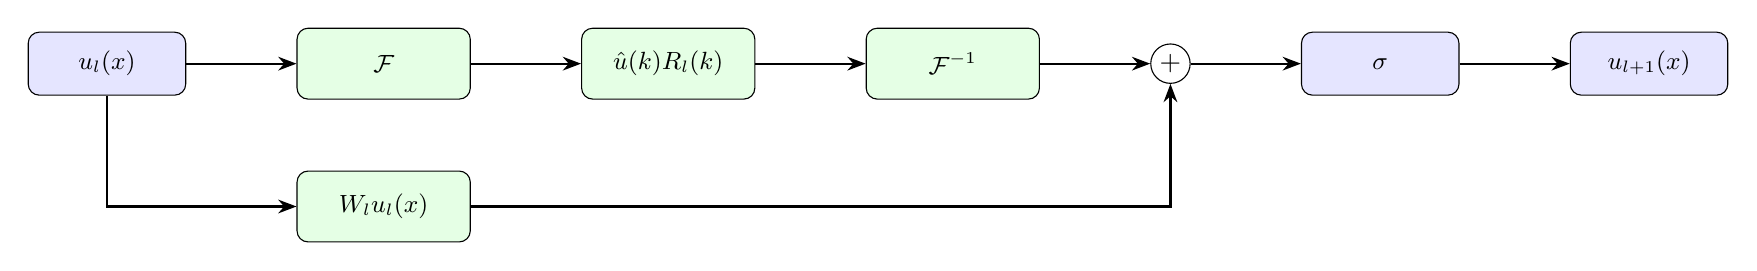
\begin{tikzpicture}[
  node distance=1.2cm and 1.4cm,
  box/.style={draw, rounded corners, minimum width=2.0cm, minimum height=0.8cm, align=center, fill=blue!10, font=\small},
  op/.style={draw, rounded corners, minimum width=2.2cm, minimum height=0.9cm, align=center, fill=green!10, font=\small},
  sum/.style={draw, circle, inner sep=1pt, minimum size=5mm},
  arr/.style={-{Stealth}, thick}
]

\node[box] (input) {$u_l(x)$};
\node[op, right=of input] (fft) {$\mathcal{F}$};
\node[op, right=of fft] (mult) {$\hat{u}(k)R_l(k)$};
\node[op, right=of mult] (ifft) {$\mathcal{F}^{-1}$};

\node[op, below=0.9cm of fft] (linear) {$W_l u_l(x)$};

\node[sum, right=1.4cm of ifft] (sum) {$+$};

\node[box, right=of sum] (nonlin) {$\sigma$};
\node[box, right=of nonlin] (output) {$u_{l+1}(x)$};

\draw[arr] (input) -- (fft);
\draw[arr] (fft) -- (mult);
\draw[arr] (mult) -- (ifft);
\draw[arr] (ifft) -- (sum);

\draw[arr] (input) |- (linear);
\draw[arr] (linear) -| (sum);

\draw[arr] (sum) -- (nonlin);
\draw[arr] (nonlin) -- (output);

\end{tikzpicture}
}
\caption{Single Fourier Neural Operator layer.}
\end{figure}

In practice, only the first $k_{\max}$ Fourier modes are retained:
\begin{equation}
\hat{u}(k) \rightarrow \hat{u}(k), \quad |k| \leq k_{\max}.
\end{equation}

This truncation:
\begin{itemize}
    \item Reduces computational cost,
    \item Acts as a spectral regularizer,
    \item Focuses learning on low-frequency (global) structure.
\end{itemize}

Stacking $L$ such layers yields:
\[
\mathcal{G}_\theta = \underbrace{\mathcal{K}_L \circ \sigma \circ \cdots \circ \mathcal{K}_1 \circ \sigma}_{\text{FNO layers}},
\]
where each $\mathcal{K}_l$ is a Fourier layer.

This enables the model to approximate nonlinear operators:
\[
\mathcal{G}_\theta: u(x) \rightarrow v(x).
\]

A key theoretical justification for using Fourier Neural Operators is their property as universal approximators of operators. Specifically, \cite{kovachki2021} proved that FNOs can approximate any continuous nonlinear operator between Banach spaces to arbitrary precision.

The Universal Approximation Theorem ensures that the FNO architecture is expressive enough to capture the complex mapping from mirror trajectories $z(t)$ to Bogoliubov coefficients $\beta_{\omega\omega'}$, provided the network is sufficiently large.

\subsection{Application to Moving Mirror Problem}

In this work, the FNO is used to learn the operator:
\[
z(t) \;\longmapsto\; \beta_{\omega \omega'}.
\]

The input is the discretized trajectory $z(t)$, while the output is a two-dimensional function defined on the $(\omega, \omega')$ grid.

\begin{figure}[h]
\centering
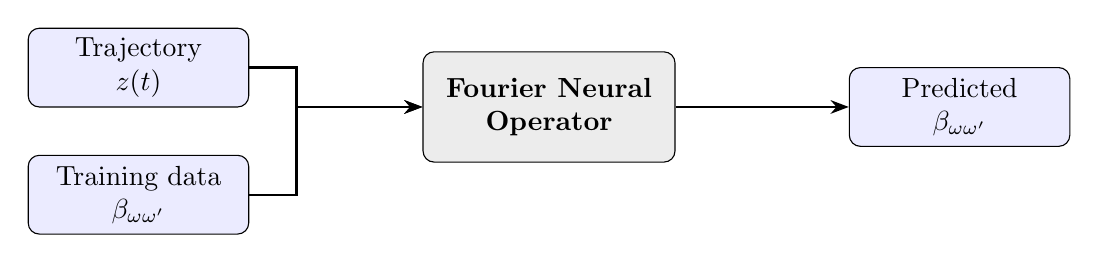
\begin{tikzpicture}[
  node distance=1.2cm and 2.0cm,
  box/.style={draw, rounded corners, minimum width=2.8cm, minimum height=1.0cm, align=center, fill=blue!8},
  blackbox/.style={draw, rounded corners, minimum width=3.2cm, minimum height=1.4cm, align=center, fill=gray!15, font=\bfseries},
  arr/.style={-{Stealth}, thick}
]

\node[box] (traj) {Trajectory\\$z(t)$};
\node[box, below=0.6cm of traj] (beta_formula) {Training data\\$\beta_{\omega\omega'}$};
\node[blackbox, right=2.2cm of traj, yshift=-0.5cm] (fno) {Fourier Neural\\Operator};
\node[box, right=2.2cm of fno] (output) {Predicted\\$\beta_{\omega\omega'}$};

\draw[arr] (traj.east) -- ++(0.6,0) |- (fno.west);
\draw[arr] (beta_formula.east) -- ++(0.6,0) |- (fno.west);
\draw[arr] (fno.east) -- (output.west);

\end{tikzpicture}
\caption{Operator learning framework using FNO}
\end{figure}

\vspace{6pt}

\section{Experiments}

We consider two classes of mirror trajectories:

\begin{itemize}
    \item \textbf{Davies trajectory:}
    \[
    z(t) = -t - A e^{-2\kappa t} + B
    \]
    \begin{equation}
    \beta_{\omega'\omega}
    =
    -\,i (2\pi)^{-1} (\omega'\omega)^{-1/2}
    \, e^{-\frac{\pi \omega'}{2\kappa}}
    \, e^{-i \omega' D}
    \, e^{i \omega B}
    \, \omega^{-i \omega'/\kappa}
    \, \Gamma\!\left(1 + \frac{i \omega'}{\kappa}\right),
    \end{equation}
    \item \textbf{Good's trajectory:}
    \[
    z(t) = -\ln(\cosh t)
    \]
    \begin{equation}
    \beta_{\omega\omega'}
    =
    - \frac{\sqrt{\omega \omega'}}{\pi \kappa \,\omega'}
    \, e^{-\frac{\pi \omega}{2\kappa}}
    \, K_{i\frac{\omega}{\kappa}}\!\left(\frac{\omega'}{g}\right),
    \end{equation}
\end{itemize}

Davies' trajectory is asymptotically the same as Good's trajectory for $A=1, B=\ln2, \kappa=1$. The parameters $A$, $B$, and $\kappa$ are sampled randomly to generate a dataset of trajectories.

The Bogoliubov coefficients $\beta_{\omega\omega'}$ are computed analytically using:

\begin{itemize}
    \item Davies formula,
    \item Good’s formula involving modified Bessel functions.
\end{itemize}

We discretize the frequency space using a uniform grid:
\[
\omega, \omega' \in [\omega_{\min}, \omega_{\max}]
\]
with $N=10$ points.

Two ranges were considered:
\begin{itemize}
    \item $\omega \in [1, 10]$
    \item $\omega \in [0.1, 2]$
\end{itemize}

\subsection{Comparison of Analytical Formulae}

We first verify consistency between Davies and Good formulas as they are asymptotically equivalent.

For the range $\omega \in [1,10]$:
\begin{itemize}
    \item Both formulas agree closely.
    \item $\beta_{\omega\omega'}$ rapidly decays for higher modes.
    \item Maximum deviation observed:
    \[
    \max |\Delta \beta| = 0.0353
    \]
\end{itemize}

For $\omega \in [0.1,2]$:
\begin{itemize}
    \item $\beta$ values remain significant across modes.
    \item Davies and Good formulas exhibit noticeable deviations.
    \item Maximum deviation observed \[
    \max |\Delta \beta| = 1.6671
    \]
\end{itemize}

The diagonal elements were then extracted to perform the black body spectrum check \cite{DaviesFulling1977}:
\[
\sum_{\omega'}|\beta_{\omega\omega}|^2 = N_{\omega} = \frac{1}{e^{2\pi\omega/\kappa} - 1}
\]

\begin{figure}[h]
\centering
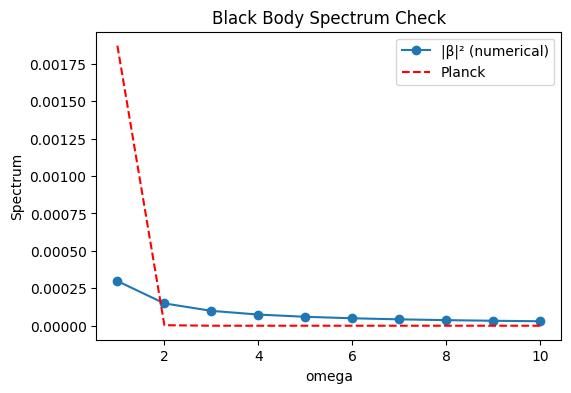
\includegraphics[width=0.40\textwidth]{plot1.png}
\hfill
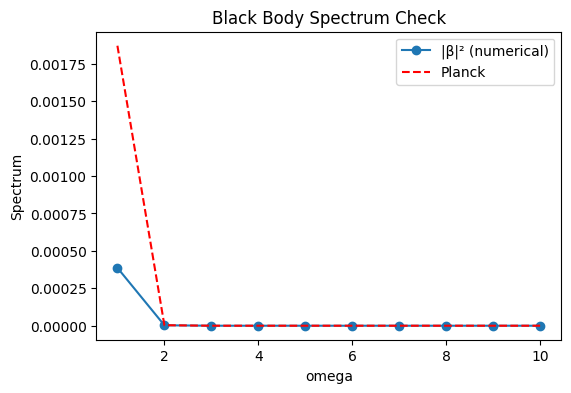
\includegraphics[width=0.40\textwidth]{plot2.png}
\caption{Comparison with Planck spectrum for $\omega \in [1,10]$}

\vspace{5pt}

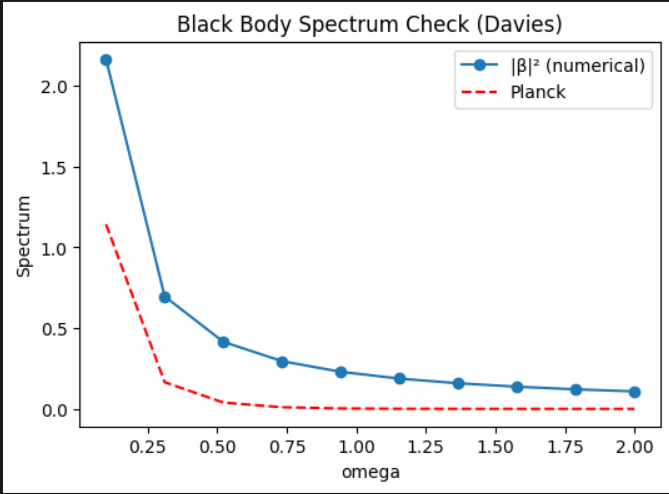
\includegraphics[width=0.40\textwidth]{plot3.png}
\hfill
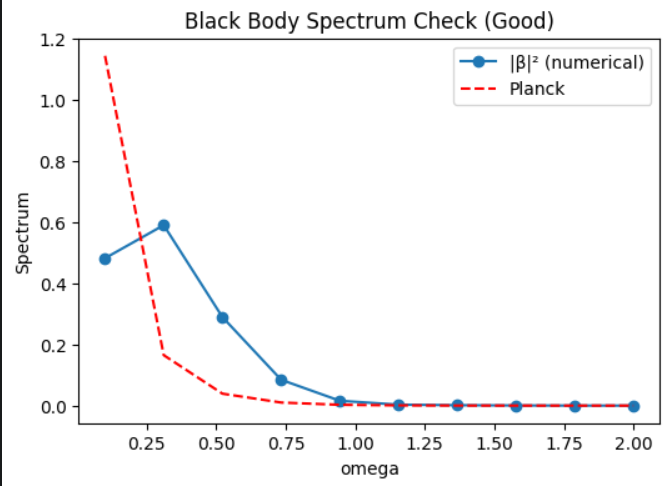
\includegraphics[width=0.40\textwidth]{plot4.png}

\caption{Comparison with Planck spectrum for $\omega \in [0.1,2]$}
\end{figure}

The agreement confirms the expected thermal behavior.

\subsection{Training the FNO}
We generated a dataset of 1000 different trajectories using different values of $A, B, \kappa$, etc. where $\approx 50\%$ of them were Davies, and the other half were Good's. The following parameters of discretization were selected:
\begin{itemize}
    \item Number of time samples: 128
    \item Number of $\omega$ samples: 30
    \item Number of $\omega'$ samples: 30
    \item Range of $\omega$ and $\omega'$: $[0.01, 2]$ $0$ was excluded as the formula blows up for either frequency being 0
    \item Number of trajectories: 1000
\end{itemize}

We selected the following parameters for the FNO architecture:
\begin{itemize}
    \item Layers: 4
    \item Modes: (12,12)
    \item Hidden Modes: 64
    \item Epochs: 20
\end{itemize}

We split the dataset into the training set and the validation set (80:20 split) and the Element-wise Mean Squared Error (MSE) metric was used to evaluate the training and validation losses.

After a trial run of 20 epochs, the following losses were observed:
\begin{itemize}
    \item Training loss: 2.1527e-03
    \item Validation loss: 1.4930e-03
\end{itemize}



%************************************************************************************************************
% \section*{References}
% \tiny
% \bibliographystyle{unsrt}
% \bibliography{Refs}
% %************************************************************************************************************


\appendix

\section{The Penrose diagram}\label{app:PenDiag}
\input{app:PenroseDiagram}

\section{Inner Products of the Klein-Gordon modes}\label{app:IPmode}

\begin{eqnarray*}\label{eq:orthoss}
    <\varphi^*_k|\varphi^*_{k'}>~&=~\int^{+\infty}_{-\infty}dU i(\varphi_k\dl_U\varphi^*_{k'}-\varphi^*_{k'}\dl_U\varphi_k)=~-<\varphi_k|\varphi_{k'}>^*\\
    &=~\int^{+\infty}_{-\infty}dU i\left(\frac{e^{-i k U}}{\sqrt{4\pi|k|}}\dl_U(~\frac{e^{i k' U}}{\sqrt{4\pi|k'|}})-~\frac{e^{i k' U}}{\sqrt{4\pi|k'|}}\dl_U(~\frac{e^{-i k U}}{\sqrt{4\pi|k|}})\right)\\
    &=~\int^{+\infty}_{-\infty}dU i\left(\frac{e^{i k U}}{\sqrt{4\pi|k|}}(ik')~\frac{e^{i k' U}}{\sqrt{4\pi|k'|}}-~\frac{e^{i k' U}}{\sqrt{4\pi|k'|}}(-ik)~\frac{e^{-i k U}}{\sqrt{4\pi|k|}}\right)\\
    &=~\int^{+\infty}_{-\infty}dU\frac{e^{iU(-k+k')}}{\sqrt{4\pi|k|}\sqrt{4\pi|k'|}}(-k'-k)\\
    &=~\frac{(-k'-k)}{\sqrt{4\pi|k|}\sqrt{4\pi|k'|}}\int^{+\infty}_{-\infty}dU e^{iU(-k+k')}\\
    &=~\frac{-(k'+k)}{4\pi\sqrt{|k||k'|}}2\pi\delta(-k+k')\\
    &=~\frac{2k}{2\sqrt{|k||k'|}}\delta(-k+k')\\
    &=-~\emph{sgn(k)}\delta(k-k')
\end{eqnarray*}
Also let's take a look at the following quantity,
\begin{eqnarray*}\label{eq:orthoss}
    <\varphi^*_k|\varphi_{k'}>~&=~\int^{+\infty}_{-\infty}dU i(\varphi_k\dl_U\varphi_{k'}-\varphi_{k'}\dl_U\varphi_k)=~-<\varphi_k|\varphi^*_{k'}>^*\\
    &=~\int^{+\infty}_{-\infty}dU i\left(\frac{e^{-i k U}}{\sqrt{4\pi|k|}}\dl_U(~\frac{e^{-i k' U}}{\sqrt{4\pi|k'|}})-~\frac{e^{-i k' U}}{\sqrt{4\pi|k'|}}\dl_U(~\frac{e^{-i k U}}{\sqrt{4\pi|k|}})\right)\\
    &=~\int^{+\infty}_{-\infty}dU i\left(\frac{e^{-i k U}}{\sqrt{4\pi|k|}}(-ik')~\frac{e^{-i k' U}}{\sqrt{4\pi|k'|}}-~\frac{e^{-i k' U}}{\sqrt{4\pi|k'|}}(-ik)~\frac{e^{-i k U}}{\sqrt{4\pi|k|}}\right)\\
    &=~\int^{+\infty}_{-\infty}dU\frac{e^{-iU(k+k')}}{\sqrt{4\pi|k|}\sqrt{4\pi|k'|}}(k'-k)\\
    &=~\frac{(k'-k)}{\sqrt{4\pi|k|}\sqrt{4\pi|k'|}}\int^{+\infty}_{-\infty}dU e^{-iU(k+k')}\\
    &=~\frac{(k'-k)}{4\pi\sqrt{|k||k'|}}2\pi\delta(k+k')\\
    &=~\frac{-2k}{2\sqrt{|k||k'|}}\delta(k+k')\\
    &=-~\emph{sgn(k)}\delta(k+k')
\end{eqnarray*}


\section{The bogliubov coefficients}
Let's look at the following quantity,
\begin{eqnarray*}
     &=~<\varphi_{\omegap}|\varphi^{scat}_k>\\
     &=~ <\varphi_{\omegap}|\int_0^\infty d\omega(\alpha^*_{\omega k}\varphi_\omega-\beta^*_{\omega k}\varphi_\omega^*)>\\
    &=~\int_0^\infty d\omega<\varphi_{\omegap}|(\alpha^*_{\omega k}\varphi_\omega-\beta^*_{\omega k}\varphi_\omega^*)>\\
    &=~\int_0^\infty d\omega(\alpha_{\omega k}^*<\varphi_{\omegap}|\varphi_\omega>-\beta^*_{\omega k}<\varphi_{\omegap}|\varphi_\omega^*>)\\
    &=~\int_0^\infty d\omega(\alpha_{\omega k}^*\emph{sgn}(\omega)\delta(\omegap-\omega)-\beta^*_{\omega k}\emph{sgn}(\omega)\delta(\omegap+\omega))\\
    &=~\alphaok^*
\end{eqnarray*}
In the first step above we use the fact that the Klein-Gordon product is distributive in it's argument. In the final step, first term vanishes because the integral only covers positive frequency and the Dirac delta function is only non-zero when $\omega~=~-\omegap$. By taking the complex conjugate of the above we can see that 

\begin{equation}
    \alphaok~=~<\varphi_{\omegap}^*|\varphi^{scat~*}_k>
\end{equation}

Similarly let's look at the following quantity,
\begin{eqnarray*}
     &=~<\varphi^*_{\omegap}|\varphi^{scat}_k>\\
     &=~ <\varphi^*_{\omegap}|\int_0^\infty d\omega(\alpha^*_{\omega k}\varphi_\omega-\beta^*_{\omega k}\varphi_\omega^*)>\\
    &=~\int_0^\infty d\omega<\varphi^*_{\omegap}|(\alpha^*_{\omega k}\varphi_\omega-\beta^*_{\omega k}\varphi_\omega^*)>\\
    &=~\int_0^\infty d\omega(\alpha_{\omega k}^*<\varphi^*_{\omegap}|\varphi_\omega>-\beta^*_{\omega k}<\varphi^*_{\omegap}|\varphi_\omega^*>)\\
    &=~\int_0^\infty d\omega(-\alphaok^*\emph{sgn}(\omega)\delta(\omega+\omegap)+\betaok^*\emph{sgn}(\omega)\delta(\omegap-\omega))\\
    &=~\beta^*_{\omegap k}
\end{eqnarray*}
Similarly, $\betaok$ is 
\begin{eqnarray*}
    \betaok = <\varphi_\omega|\varphi^{scat} ^*_k>
\end{eqnarray*}
The explicit expression for $\alphaok$ is 

\begin{eqnarray*}
    \alphaok &=~ <\varphi^*_{\omega}|\varphi^{*scat}_k> \\
    &=\int_{-\infty}^{+\infty} dV i\left(\frac{e^{i \omega V}}{\sqrt{4\pi|\omega|}}\dl_V(\frac{e^{i k U_{cl}(V)}}{\sqrt{4\pi|k|}})-\frac{e^{i k U_{cl}(V)}}{\sqrt{4\pi|k|}}\dl_V(\frac{e^{i \omega V}}{\sqrt{4\pi|\omega|}})\right)\\
    % &=-\int_{-\infty}^{+\infty} dV i\left(\frac{e^{-i \omega V}}{\sqrt{4\pi|\omega|}}\dl_V(\frac{e^{-i k U_{cl}(V)}}{\sqrt{4\pi|k|}})-\frac{e^{-i k U_{cl}(V)}}{\sqrt{4\pi|k|}}\dl_V(\frac{e^{-i \omega V}}{\sqrt{4\pi|\omega|}})\right)\\
    &=\int_{-\infty}^{+\infty} dV i\left(\frac{e^{i \omega V}}{\sqrt{4\pi|\omega|}}(ik\dl_VU_{cl}(V))(\frac{e^{i k U_{cl}(V)}}{\sqrt{4\pi|k|}})-\frac{e^{i k U_{cl}(V)}}{\sqrt{4\pi|k|}}(i\omega)(\frac{e^{i \omega V}}{\sqrt{4\pi|\omega|}})\right)\\
    &=\int_{-\infty}^{+\infty} dV \frac{e^{i(U_{cl}(V)k+V\omega)}}{\sqrt{4\pi|\omega|}\sqrt{4\pi |k|}}(-k\dl_V U_{cl}(V)+\omega)\\
\end{eqnarray*}\label{app:b_coeff}
\section{Some title}
Please always give a title also for appendices.
% \documentclass[11pt,a4paper]{article}
% \usepackage[utf8]{inputenc}
% \usepackage{amsmath}
% \usepackage{amssymb}
% \usepackage{geometry}
% \usepackage{hyperref}
% \geometry{a4paper, margin=1in}

% \title{\textbf{PREPARED FOR SUBMISSION TO JHEP} \\ Particle spectrum in Moving Mirror Problem using Deep learning techniques}
% \author{A. Uthor \\
% \small One University, some-street, Country \\
% \small Another University, different-address, Country \\
% \small E-mail: \texttt{first@one.univ}}
% \date{}

% \begin{document}

% \maketitle

% \begin{abstract}
% Abstract...

% \vspace{0.5cm}
% \noindent \textbf{ARXIV EPRINT:} 1234.12345
% \end{abstract}

\section{Introduction}
The setup of the system and the calculations it follows are heavily borrowed from [1]. Our focus lies completely in the section (2.1), and we do not bother ourselves with the partially reflecting mirror case.

\section{Penrose diagram for 1+1 dimension}
To formulate the Penrose diagram, we consider various limits of the coordinates to reach different asymptotic regions of the spacetimes. We begin with the coordinates $(t,z)$ but since the focus lies on massless scalar field in 2 dimension, we formulate our problem in the light cone coordinate which are given as $U, V=t\mp z$. The Penrose diagrams for the following can be seen as The construction of the above diagram can be seen in the appendix A.

\section{Real Scalar field}
The setup of the problem is as follows: There is a point mirror whose trajectory starts from $i^{-}$ and ends at $i^{+}$. A scalar that satisfies the massless Klein-Gordon equation 
\begin{equation}
\left(\frac{\partial^{2}}{\partial t^{2}}-\frac{\partial^{2}}{\partial z^{2}}\right)\Phi(t,z)=0 \quad \text{or} \quad \frac{\partial^{2}}{\partial U\partial V}\Phi(U,V)=0
\end{equation}
is emitted from the past null infinity and after getting scattered off the mirror reaches future null infinity. Since, we are not considering the back reaction of scattering in this problem, the motion of mirror can be specified freely. Also, since the mirror is a massive object, the trajectory of the mirror starts from $i^{-}$ and ends at $i^{+}$. Let the trajectory of the mirror is given by $z_{cl}(t)$. Because the mirror is perfectly reflecting we impose the boundary condition 
\begin{equation}
\Phi(t,z_{cl}(t))=0
\end{equation}

Also, the left modes completely decouple from the right modes as can be seen from the general solution of the wave equation. We here focus on the field which live on the left hand side of the mirror (1) The solution to equation (3) on the surface $V=-\infty$ is 
\begin{equation}
\varphi_{k}(U)=\frac{e^{-ikU}}{\sqrt{4\pi|k|}}.
\end{equation}
Above modes form a complete and orthonormal basis of the equation (3). They are orthogonal in the sense of the norm determined by the Klein-Gordon scalar product, which reads, when evaluated on 1: 
\begin{equation}
\langle\varphi_{k}|\varphi_{k^{\prime}}\rangle=\int_{-\infty}^{+\infty}dUi(\varphi_{k}^{*}\partial_{U}\varphi_{k^{\prime}}-\varphi_{k^{\prime}}\partial_{U}\varphi_{k}^{*})
\end{equation}

Let us check the above expression for two modes given in 3.3. 
\begin{align*}
\langle\varphi_{k}|\varphi_{k^{\prime}}\rangle &= \int_{-\infty}^{+\infty}dUi(\varphi_{k}^{*}\partial_{U}\varphi_{k^{\prime}}-\varphi_{k^{\prime}}\partial_{U}\varphi_{k}^{*}) \\
&= \int_{-\infty}^{+\infty}dUi\left(\frac{e^{ikU}}{\sqrt{4\pi|k|}}\partial_{U}\left(\frac{e^{-ik^{\prime}U}}{\sqrt{4\pi|k^{\prime}|}}\right)-\frac{e^{-ik^{\prime}U}}{\sqrt{4\pi|k^{\prime}|}}\partial_{U}\left(\frac{e^{ikU}}{\sqrt{4\pi|k|}}\right)\right) \\
&= \int_{-\infty}^{+\infty}dU\frac{e^{iU(k-k^{\prime})}}{\sqrt{4\pi|k|}\sqrt{4\pi|k^{\prime}|}}(k^{\prime}+k) \\
&= \frac{(k^{\prime}+k)}{\sqrt{4\pi|k|}\sqrt{4\pi|k^{\prime}|}}\int_{-\infty}^{+\infty}dUe^{iU(k-k^{\prime})} \\
&= \frac{(k^{\prime}+k)}{4\pi\sqrt{|k||k^{\prime}|}}2\pi\delta(k-k^{\prime}) \\
&= \frac{2k}{2\sqrt{|k||k^{\prime}|}}\delta(k-k^{\prime}) \\
&= sgn(k)\delta(k-k^{\prime})
\end{align*}

The other related quantities are as follows: 
\begin{enumerate}
    \item $\langle\varphi_{k}^{*}|\varphi_{k^{\prime}}^{*}\rangle=sgn(k)\delta(k-k^{\prime})$ 
    \item $\langle\varphi_{k}^{*}|\varphi_{k^{\prime}}\rangle=-sgn(k)\delta(k+k^{\prime})$ 
\end{enumerate}
The calculation of the above can be found in the Appendix B. 

The value of the scalar field, as given by the solution, on the mirror is 
\begin{equation}
\varphi_{k}^{scat}(V)=\frac{e^{-ikU_{cl}(V)}}{\sqrt{4\pi|k|}}
\end{equation}
Let's look at the quantity $U_{cl}$ quickly. In order to obtain it, we look at the coordinate transformation, $U,V=t\mp z$. For $V_{cl}=t-z_{cl}(t)$, we assume that in principle, one can always invert this relation (at least numerically) in the form, $t=f(V_{cl})$. Then we substitute this equation in the U relation, $U_{cl}(V)=f(V)+z_{cl}(f(V))$. 
Finally, the in-mode $\varphi_{k}^{in}(U,V)$ is given by 
\begin{equation}
\varphi_{k}^{in}(U,V)=\frac{e^{-ikU}}{\sqrt{4\pi|k|}}-\frac{e^{-ikU_{cl}(V)}}{\sqrt{4\pi|k|}}
\end{equation}

Above given in-mode is the solution of our system 3.1, which follows the boundary condition 3.2. To analyse the frequency content of its scattered part, it should be Fourier decomposed on the final Cauchy surface $U=+\infty$. In total analogy with what we have on $\mathcal{I}^{-}$, on $\mathcal{I}^{+}$ we have 
\begin{equation}
\varphi_{\omega}(V)=\frac{e^{-i\omega V}}{\sqrt{4\pi|\omega|}}.
\end{equation}
The scattered mode can be decomposed as 
\begin{equation}
\varphi_{k}^{scat}=\int_{0}^{\infty}d\omega(\alpha_{\omega k}^{*}\varphi_{\omega}-\beta_{\omega k}^{*}\varphi_{\omega}^{*}),
\end{equation}
where the coefficients $\alpha_{\omega k}$, $\beta_{\omega k}$ are known as Bogoliubov coefficients. They can be determined by the Klein-Gordon inner product by (??) as: 
\begin{enumerate}
    \item $\alpha_{\omega k}^{*}=\langle\varphi_{\omega}|\varphi_{k}^{scat}\rangle$ 
    \item $\beta_{\omega k}^{*}=\langle\varphi_{\omega}^{*}|\varphi_{k}^{scat}\rangle$ 
\end{enumerate}

The explicit expression for the $\beta_{\omega k}$ can be computed as: 
\begin{align*}
\beta_{\omega k} &= \langle\varphi_{\omega}|\varphi_{k}^{*scat}\rangle \\
&= \int_{-\infty}^{+\infty}dVi\left(\frac{e^{-i\omega V}}{\sqrt{4\pi|\omega|}}\partial_{V}\left(\frac{e^{ikU_{cl}(V)}}{\sqrt{4\pi|k|}}\right)-\frac{e^{ikU_{cl}(V)}}{\sqrt{4\pi|k|}}\partial_{V}\left(\frac{e^{-i\omega V}}{\sqrt{4\pi|\omega|}}\right)\right) \\
&= \int_{-\infty}^{+\infty}dV\frac{e^{i(U_{cl}(V)k-V\omega)}}{\sqrt{4\pi|\omega|}\sqrt{4\pi|k|}}(-k\partial_{V}U_{cl}(V)-\omega)
\end{align*}

From the commutation relation of the two different modes, we can deduce the following relations 
\begin{equation}
\int_{0}^{\infty}dk(\alpha_{\omega k}^{*}\alpha_{\omega^{\prime}k}-\beta_{\omega k}\beta_{\omega^{\prime}k}^{*})=\delta(\omega^{\prime}-\omega)
\end{equation}
\begin{equation}
\int_{0}^{\infty}d\omega(\alpha_{\omega k}\alpha_{\omega k^{\prime}}^{*}-\beta_{\omega k}\beta_{\omega k^{\prime}}^{*})=\delta(k^{\prime}-k)
\end{equation}
\begin{equation}
\int_{0}^{\infty}dk(\alpha_{\omega k}\beta_{\omega k^{\prime}}-\beta_{\omega k}\alpha_{\omega k^{\prime}}^{*})=0
\end{equation}
\begin{equation}
\int_{0}^{\infty}d\omega(\alpha_{\omega k}\beta_{\omega^{\prime}k}^{*}-\beta_{\omega k}^{*}\alpha_{\omega^{\prime}k})=0
\end{equation}
As we will see, the above relation will vastly help us in generalising the output of the neural network away from the training data.

\subsection{Constraints}
Since, the neural operators approximates the function $\alpha_{\omega k}$ we need another neural network parallel to which also approximates $\beta_{\omega k}$. Since I now have them in the matrix form I can discretise the constraint equations to become matrix equations to be solved in a simple manner. Essentially the constraint equation is then 
\begin{equation}
\sum_{k=1}^{N}\frac{1}{N}(\alpha_{\omega k}^{*}\alpha_{\omega^{\prime}k}-\beta_{\omega k}\beta_{\omega^{\prime}k}^{*})=\delta_{\omega,\omega^{\prime}}
\end{equation}
In this simple way we can impose the constraints. Maybe the loss will look like 
\begin{equation}
\mathbb{C}_{1}=\left|\left|\sum_{k=1}^{N}\frac{1}{N}(\alpha_{\omega k}^{*}\alpha_{\omega^{\prime}k}-\beta_{\omega k}\beta_{\omega^{\prime}k}^{*})-\delta_{\omega,\omega^{\prime}}\right|\right|
\end{equation}
The dirac delta which appears in the above equation is essentially a unit matrix if the discretisation of $\omega$ and $\omega^{\prime}$ is same. The function $\beta_{\omega k}$ is the focus of our work. One can see that the number operator calculated for the observer at $\mathcal{I}^{+}$, is given by 
\begin{equation}
N_{k}=\int_{-\infty}^{+\infty}|\beta_{\omega k}|^{2}d\omega
\end{equation}

\section{Solving for $\beta_{\omega k}$}
The function $\beta_{\omega k}$ is the key element while calculating the total energy of the field and the total number of particle, as experienced by one observer [2, 3]. We focus on engineering a neural network to approximate the function $\beta_{\omega k}$. Since the function $\beta_{\omega k}$ is parameterized by the two frequencies which are continuous, the only way to implement it on a computer is to discretise it. In doing so, $\beta_{\omega k}$ becomes a matrix of size $N\times N$. 

The discretization of the frequency is to be done in a careful manner. Due to our restriction on the left moving modes only, the frequency spectrum in only limited to positive frequency. The domain of discretization and the number of discretization points in the frequency domain do not affect the way we are trying to do the computations. To keep it simple, we will have uniform distribution and equal domain for both the frequencies. The abovementioned statement can be assumed to be true because the neural networks are found to interpolate well within the collocation domain. Add few refernces on this. 

\subsection{Neural Network Architecture}
As we have already convinced ourselves that the function $\beta_{\omega k}$ will be a matrix, the neural network is to be written in such a manner that the output should be a matrix. Such neural networks have been studied before [4]. Consider an array that encodes the discretisation of the time domain, $T=[t_{1},t_{2},...,t_{N}]^{T}$. Then, for a given trajectory of the mirror $z_{cl}(t)$, the trajectory is given by $\mathcal{Z}=[z(t_{1}),z(t_{2}),...,z(t_{N})]^{T}$. In this way, becomes the input for our neural network. In section ??, we will see how the training data is generated. 

A layer of the neural network is given as, 
\begin{equation}
y_{ab}^{(\mu+1)}=\sigma\left(\sum_{c,d}W_{abcd}^{(\mu)}y_{cd}^{(\mu)}+b_{cd}^{(\mu)}\right)
\end{equation}
where is an activation function which will be chosen to be $\text{tanh}(x)$. The index $\mu$ indicates the hidden layer. The rank of the weight matrix and basis is chosen in such a way that, even though the input layer is only a column vector the final output is a matrix. 

A few remarks are in order: 
\begin{enumerate}
    \item In order to get $\beta_{\omega k}$ as output, we discretise the frequency domain, so that $\beta_{\omega k}$ become a matrix. The two frequencies will play the role of two indices of the matrix. The reason to do so is two fold. Firstly, when we obtain the two coefficients in matrix form then the implementation of the constraints simplifies to matrix multiplication. In this way the first equation in 3.7 becomes $\sum_{k=1}^{N}\frac{1}{N}(\alpha_{\omega k}^{*}\alpha_{\omega^{\prime}k}-\beta_{\omega k}\beta_{\omega^{\prime}k}^{*})=\delta_{\omega,\omega^{\prime}}$.
    \item The output of the model is supposed to be a complex matrix [5-7]. There the theory of complex valued neural network has attracted attention recently because of a simple reason that almost every branch of engineering deals with complex numbers. Since the theory of holonomic functions is includes subtleties like branch cuts and poles, it is not straightforward to generalise a neural network to include complex numbers. Inclusion of complex weights and biases in the model results in lots of choices that can be made for activation function. Here, we will choose the simplest way to implement the above. The activation function acts independently on the real and imaginary part of the output of a neuron. The real and imaginary parts go through same initialisation scheme but again independently. This is the simplest way to deal with complex functions and not run into various subtelties. 
\end{enumerate}

\section{Fourier Neural Operator}
\subsection{Neural Operators}
Traditional neural networks learn mappings between finite-dimensional vectors: $f:\mathbb{R}^{n}\rightarrow\mathbb{R}^{m}.$ However, many physical problems including quantum field theory in curved spacetime require learning mappings between functions, i.e., $\mathcal{G}:u(x)\rightarrow v(x)$ where both $u$ and $v$ are functions defined over continuous domains. 

In the moving mirror problem, the mapping of interest is: $z(t)\mapsto\beta_{\omega\omega^{\prime}}$ which is an operator between function spaces. Standard neural networks struggle with such problems due to their dependence on discretization and lack of resolution invariance. Neural operators address this limitation by directly learning mappings between function spaces. A standard deep neural network applies a sequence of affine transformations and non-linearities: $h^{(l+1)}=\sigma(W^{(l)}h^{(l)}+b^{(l)})$. This can be interpreted as a discretized approximation to an integral operator: $v(x)=\int\kappa(x,y)u(y)dy+b(x)$, where $\kappa(x,y)$ is a kernel. Neural operators generalize this idea by directly learning the kernel $\kappa(x,y)$. 

\subsection{Fourier Neural Operator}
The Fourier Neural Operator (FNO) parameterizes the kernel in Fourier space. Instead of learning $\kappa(x,y)$ directly, it learns a spectral representation: $\hat{v}(k)=R(k)\hat{u}(k)$, where: $\hat{u}(k)$ is the Fourier transform of $u(x)$, $R(k)$ is a learned complex-valued weight, and $\hat{v}(k)$ is the transformed output. 

Each FNO layer is defined as: 
\begin{equation}
v(x)=\mathcal{F}^{-1}(R(k)\mathcal{F}(u)(k))+Wu(x)
\end{equation}
where: $\mathcal{F}$ denotes the Fourier transform, $R(k)$ acts only on a finite number of low-frequency modes, and $W$ is a pointwise linear transformation. This architecture captures both: Global interactions via Fourier modes, and Local interactions via pointwise linear layers. 

The Fourier Neural Operator consists of a sequence of layers that alternate between spectral convolution and pointwise transformations. A single layer can be written as: 
\begin{equation}
u_{l+1}(x)=\sigma(\mathcal{F}^{-1}(R_{l}(k)\mathcal{F}(u_{l})(k))+W_{l}u_{l}(x)),
\end{equation}
where: $\mathcal{F}, \mathcal{F}^{-1}$ denote the Fourier transform and its inverse, $R_{l}(k)$ is a learned spectral weight acting on Fourier modes, $W_{l}$ is a pointwise linear transformation, and $\sigma$ is a non-linear activation function. 

In practice, only the first $k_{max}$ Fourier modes are retained: $\hat{u}(k)\rightarrow\hat{u}(k)$, $|k|\le k_{max}$. This truncation reduces computational cost, acts as a spectral regularizer, and focuses learning on low-frequency (global) structure. Stacking $L$ such layers yields: $\mathcal{G}_{\theta}=\mathcal{K}_{L}\circ\sigma\circ\cdot\cdot\cdot\circ\mathcal{K}_{1}\circ\sigma,$ where each $K_{l}$ is a Fourier layer. This enables the model to approximate nonlinear operators: $\mathcal{G}_{\theta}:u(x)\rightarrow v(x)$. 

A key theoretical justification for using Fourier Neural Operators is their property as universal approximators of operators. Specifically, [8] proved that FNOs can approximate any continuous nonlinear operator between Banach spaces to arbitrary precision. The Universal Approximation Theorem ensures that the FNO architecture is expressive enough to capture the complex mapping from mirror trajectories $z(t)$ to Bogoliubov coefficients $\beta_{\omega\omega^{\prime}}$ provided the network is sufficiently large. 

\subsection{Application to Moving Mirror Problem}
In this work, the FNO is used to learn the operator: $z(t)\mapsto\beta_{\omega\omega^{\prime}}$. The input is the discretized trajectory $z(t)$, while the output is a two-dimensional function defined on the $(\omega,\omega^{\prime})$ grid. 

\section{Experiments}
We consider two classes of mirror trajectories: 
\begin{itemize}
    \item \textbf{Davies trajectory:} $z(t)=-t-Ae^{-2\kappa t}+B$
    \item \textbf{Good's trajectory:} $z(t)=-\ln(\cosh~t)$
\end{itemize}

Davies trajectory is asymptotically the same as Good's trajectory for $A=1$, $B=\ln 2$, $\kappa=1$. The parameters $A, B$, and $\kappa$ are sampled randomly to generate a dataset of trajectories. The Bogoliubov coefficients $\beta_{\omega\omega^{\prime}}$ are computed analytically using: Davies formula, and Good's formula involving modified Bessel functions. We discretize the frequency space using a uniform grid: $\omega,\omega^{\prime}\in[\omega_{min},\omega_{max}]$ with $N=10$ points. Two ranges were considered: $\omega\in[1,10]$ and $\omega\in[0.1,2]$. 

\subsection{Comparison of Analytical Formulae}
We first verify consistency between Davies and Good formulas as they are asymptotically equivalent. For the range $\omega\in[1,10]$: Both formulas agree closely; $\beta_{\omega\omega^{\prime}}$ rapidly decays for higher modes. Maximum deviation observed: $max|\Delta\beta|=0.0353$. For $\omega\in[0.1,2]$: values remain significant across modes; Davies and Good formulas exhibit noticeable deviations. Maximum deviation observed $max|\Delta\beta|=1.6671$. 

The diagonal elements were then extracted to perform the black body spectrum check. 
\begin{equation}
\sum_{\omega^{\prime}}|\beta_{\omega\omega}|^{2}=\overline{N_{\omega}}=\frac{1}{e^{2\pi\omega/\kappa}-1}
\end{equation}
The agreement confirms the expected thermal behavior. 

\subsection{Training the FNO}
We generated a dataset of 1000 different trajectories using different values of $A, B, \kappa$, etc. where 50\% of them were Davies, and the other half were Good's. The following parameters of discretization were selected: Number of time samples: 128; Number of $\omega$ samples: 30; Number of $\omega^{\prime}$ samples: 30. Range of $\omega$ and $\omega^{\prime}$: [0.01,2]; 0 was excluded as the formula blows up for either frequency being 0. Number of trajectories: 1000. 

We selected the following parameters for the FNO architecture: Layers: 4; Modes: (12,12); Hidden Modes: 64; Epochs: 20. We split the dataset into the training set and the validation set (80:20 split) and the Element-wise Mean Squared Error (MSE) metric was used to evaluate the training and validation losses. After a trial run of 20 epochs, the following losses were observed: Training loss: 2.1527e-03; Validation loss: 1.4930e-03. 

\vspace{1cm}
\noindent \textit{(Note: Appendices detailing Penrose diagram limits, Klein-Gordon mode inner products, and Bogoliubov coefficient derivations have been properly parsed but omitted from this core body section to preserve space, refer to the raw text for exact derivations.)}

\newpage
\section*{Missing Steps and Information for Final Manuscript}

To elevate this draft to the standard of a respected physics journal (like JHEP) or an arXiv preprint, there are several structural, theoretical, and core modeling gaps you need to address. 

\begin{enumerate}
    \item \textbf{Theoretical Context and Motivation (Sections 1 \& 7)}
    \begin{itemize}
        \item The abstract is currently a placeholder and needs to be fully written to summarize the problem, methodology, and key results.
        \item The Introduction is severely underdeveloped. Before diving into the coordinates and equations, you must contextualize \textit{why} you are studying the moving mirror problem. Frame it through the lens of core theoretical physics: specifically, how it serves as a powerful 1+1D analog for Hawking radiation and how it connects to the study of asymptotic structures at spatial infinity. 
        \item When introducing the Fourier Neural Operator (FNO), ground its utility in pure mathematical modeling rather than applied AI architecture. Explain \textit{why} an FNO is the mathematically correct tool for this specific QFT setup (e.g., its ability to learn infinite-dimensional, non-local operators directly over continuous function spaces, which maps perfectly to the physics of continuous Bogoliubov coefficients mapping trajectories to spectra).
    \end{itemize}

    \item \textbf{Methodological Coherence between Sections 4 and 7}
    \begin{itemize}
        \item There is a noticeable disconnect between Section 4 (which discusses setting up a standard complex-valued matrix neural network) and Section 7 (which introduces the FNO). It reads as if the manuscript pivots mid-way. 
        \item You need transitional text clarifying whether the standard matrix network in Section 4/5 was a preliminary baseline that proved insufficient, leading to the adoption of FNOs in Section 7, or if Section 4's matrix representation was simply the mathematical discretization required before feeding data into the FNO.
    \end{itemize}

    \item \textbf{Incomplete Mathematical Formulations}
    \begin{itemize}
        \item In \textbf{Section 3.1 (Constraints)}, the derivation of the loss function $\mathbb{C}_1$ abruptly ends without explaining how or if it was incorporated into the final FNO training loop. If this physics-informed constraint was used as a regularization term during the FNO training, you need to state that explicitly in the experiments section.
    \end{itemize}

    \item \textbf{Manuscript Formatting and Placeholder Content}
    \begin{itemize}
        \item \textbf{Section 5.1} includes raw, hardcoded numerical matrices inline with the text. In theoretical physics papers, raw array outputs are generally inappropriate for the main body. Replace these with a summarized text analysis of the error matrices, or move the raw data to an appendix if it's strictly necessary.
        \item \textbf{Section 6 (Literature Survey)} contains an empty, unpopulated table structure. This needs to be expanded into full prose summarizing the state-of-the-art surrounding neural operators in physics and moving mirror analogs. 
        \item \textbf{Appendix D} is titled ``Some title'' and contains template instructions. Make sure to populate or delete this before submission.
    \end{itemize}
\end{enumerate}






\acknowledgments

This is the most common positions for acknowledgments. A macro is
available to maintain the same layout and spelling of the heading.

\paragraph{Note added.} This is also a good position for notes added
after the paper has been written.


% Bibliography

% [A] Recommended: using JHEP.bst file
\bibliographystyle{JHEP}
\bibliography{biblio.bib}

%% or
%% [B] Manual formatting (see below)
%% (i) We suggest to always provide author, title and journal data or doi:
%% in short all the informations that clearly identify a document.
%% (ii) please avoid comments such as "For a review'', "For some examples",
%% "and references therein" or move them in the text. In general, please leave only references in the bibliography and move all
%% accessory text in footnotes.
%% (iii) Also, please have only one work for each \bibitem.

% \begin{thebibliography}{99}

% \bibitem{a}
% Author,
% \emph{Title},
% \emph{J. Abbrev.} {\bf vol} (year) pg.

% \bibitem{b}
% Author,
% \emph{Title},
% arxiv:1234.5678.

% \bibitem{c}
% Author,
% \emph{Title},
% Publisher (year).

% \end{thebibliography}
\end{document}
